\documentclass{TDP005mall}
\usepackage{graphicx}
\newcommand{\version}{Version 1.0}
\author{Agnes Hallberg, \url{agnha531@student.liu.se}\\
  Eric Jönsson, \url{erijo137@student.liu.se}}
\title{Designspecifikation}
\date{2018-11-27}
\rhead{Agnes Hallberg\\
  Eric Jönsson\\}
\begin{document}
\projectpage

\section*{Revisionshistorik}
\begin{table}[!h]
\begin{tabularx}{\linewidth}{|l|X|l|}
\hline
Ver. & Revisionsbeskrivning & Datum \\\hline
1.0 & Första utkast  & 18-11-27 \\\hline
\end{tabularx}
\end{table}

\section{Detaljbeskrivning av Player}
Playerklassen ska representera karaktären spelaren kontrollerar. Spelaren har två olika attacker att välja mellan samt tre riktningar att röra sig i. Spelkaraktären kan inte lämna spelplanen. Klassen Player ärver från överklassen Entity. Följande klassmedlemmar finns i Playerklassen:
\begin{itemize}
\item int hp; ärvs från Entity. Denna datamedlem innehåller information om hur mycket skada spelkaraktären kan ta innan förlust.
\item Vector2f position; ärvs från Entity. position sparar spelkaraktärens koordinater på banan.
\item Vector2f movespeed; ärvs från Character. Dikterar hur snabbt spelkaraktären kan röra sig per tick.
\item void player\_update().
\item void hit().
\item void jump(). Spelkaraktären rör sig i y-led till en viss y-koordinat och sedan tillbaka i motsatt riktning.
\end{itemize}
\section{Beskrivning av Enemy}
Enemyklassen ska reprensentera fienderna som spelaren behöver besegra. 
Enemyklassen har två underklasser; Peasant och Knight.
Enemy är en abstrakt klass. 
Spelkaraktären tar skada när den kolliderar med någon av fiendeobjekten. 
Fienderobjektens mål är att röra sig in i spelkaraktären. 
Enemyklassen ärver från Entityklassen.
\begin{itemize}
\item int hp; ärvs från Entity. 
    Denna datamedlem innehåller information om hur mycket skada Enemyobjektet kan ta innan destruktion.
\item Vector2f position; ärvs från Entity. 
    position sparar Enemyobjektets koordinater på banan.
\item Vector2f movespeed; ärvs från Entity. Dikterar hur snabbt Enemyobjektet kan röra sig per tick.
\item int immunity.
  Används i hit() för att avgöra om Enemyobjektet ska ta skada eller inte.
\item void hit().
    Denna funktion kallas när spelkaraktären träffar ett fiendeobjekt med en attack. 
    Om attacken inte motsvarar värdet i immunity tar fienden skada.
\end{itemize}
\subsection{Peasant}
Peasant är den vanligaste förekommande fiendetypen och finns i två varianter. 
Det som skiljer varianterna åt är värdet i immunity. 
Texturen på fienden visar vilken immunity den har.
Peasant rör sig mot spelkaraktären. 
\subsection{Knight}
Knight ska upplevas svårare att besegra än Peasant. 
Knight rör sig långsammare än Peasant och spelkaraktären. 
Knights attack är långsam och försätter den i ett attackläge likt spelkaraktärens. 
Knight är immun mot svaga attacker. 
Knight kräver fler attacker för att besegras än andra fiendetyper.
\begin{itemize}
\item void initiate\_attack(). Denna funktion kallas när spelaren är inom räckhåll för Knights attack. 
    Knight står stilla i attackläge under hela sin attack.
\end{itemize}
\newpage

\section{Designbeskrivning}
Designen av vårt spel bygger på att vi har en central spelmotor som väljer mellan fyra olika spelstadier;
PlayState, MenuState, GameOverState samt WinState.
Vi gjorde detta designval för att enklare kunna expandera spelet med fler gamestates som till exempel cutscenes samt för att kunna komma åt data i olika spelstadier. 
Designvalet gör utveckling av spelet mer omfattande och om den tillagda funktionaliteten inte utnyttjas till fullo blir det ett slöseri av resurser.
En alternativ design hade kunnat vara att skippa spelmotorn och enbart ha två spelstadier att växla mellan.
Denna lösning har fler begränsningar men är mindre resurs- och tidskrävande.

Då klasserna Player och Enemy har gemensamma attribut väljer vi att låta dem ärva från samma abstrakta klass, Entity. 
Detta leder till mindre upprepning av kod, vilket i sin tur leder till färre buggar och tydligare kod.

När spelet körs skapar det och visar ett MenuState. 
Via Menustate kan spelaren sedan komma åt de andra spelstadierna förutom WinState och GameOverState.
När PlayState blir anropad läser den in spelplanen från fil. 
Spelplanen innehåller sitt eget utseende samt hur många fiender som behöver besegras och när de skickas in.
PlayState innehåller spelarkaraktären och en vektor av fiender som finns på spelplanen.
I varje tick kontrollerar PlayState att ingen fiende befinner sig inom spelkaraktärens hitbox. 
Om en fiende befinner sig inom spelkaraktärens hitbox kallas take\_damage() på spelkaraktären.

Vidare kommer PlayState ansvara för interaktioner mellan objekten på spelplanen samt ansvara för interaktioner mellan objekten och spelplanen.
\newpage
Följande klassdiagram visar förhållandet mellan klasserna.
\begin{figure}[h!]
    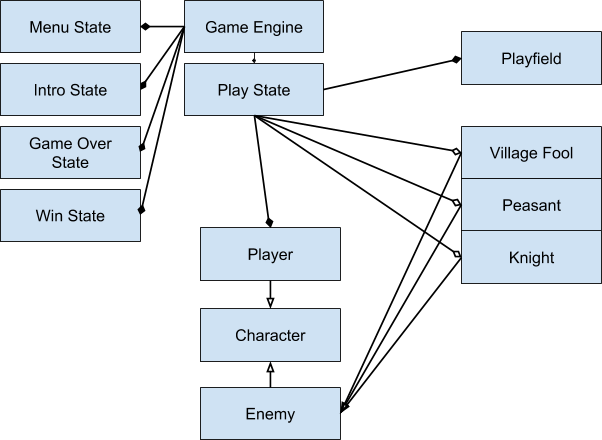
\includegraphics[width=\linewidth]{class_diagram.png}
\end{figure}
\section{Externa filer}
Spelet hanterar en extern fil för att ladda in spelplanen och för att lagra highscores på den specifika planen. 
Filen som behandlas ska vara en txt-fil. 
Den datan som behöver behandlas är spelplanens storlek, fienders startpunkter samt inskickningstider och antal. 
Vi sparar även en lista med de tre bästa highscores i samma fil så att olika banor får egna highscores.  

\end{document}
